%%%%%%%%%%%%%%%%%%%%%%%%%%%%%%%%%%%%%%%%%%%%%%%%%%%%%%%%%%%%
%%% ELIFE ARTICLE TEMPLATE
%%%%%%%%%%%%%%%%%%%%%%%%%%%%%%%%%%%%%%%%%%%%%%%%%%%%%%%%%%%%
%%% PREAMBLE 
\documentclass[9pt,lineno]{elife}
% Use the onehalfspacing option for 1.5 line spacing
% Use the doublespacing option for 2.0 line spacing
% Please note that these options may affect formatting.
% Additionally, the use of the \newcommand function should be limited.


\usepackage{lipsum} % Required to insert dummy text
\usepackage[version=4]{mhchem}
\usepackage{siunitx}
\DeclareSIUnit\Molar{M}

%%%%%%%%%%%%%%%%%%%%%%%%%%%%%%%%%%%%%%%%%%%%%%%%%%%%%%%%%%%%
%%% ARTICLE SETUP
%%%%%%%%%%%%%%%%%%%%%%%%%%%%%%%%%%%%%%%%%%%%%%%%%%%%%%%%%%%%
\title{Regulation of membrane scission in yeast endocytosis}

\author[1*]{Deepikaa Menon}
%\author[1,2\authfn{1}\authfn{3}]{Firstname Middlename Familyname}
%\author[2\authfn{1}\authfn{4}]{Firstname Initials Surname}
\author[2*]{Marko Kaksonen}
\affil[1]{Institution 1}
%\affil[2]{Institution 2}

\corr{email1@example.com}{FMS}
\corr{email2@example.com}{FS}

\contrib[\authfn{1}]{These authors contributed equally to this work}
\contrib[\authfn{2}]{These authors also contributed equally to this work}

\presentadd[\authfn{3}]{Department, Institute, Country}
\presentadd[\authfn{4}]{Department, Institute, Country}
% \presentadd[\authfn{5}]{eLife Sciences editorial Office, eLife Sciences, Cambridge, United Kingdom}

%%%%%%%%%%%%%%%%%%%%%%%%%%%%%%%%%%%%%%%%%%%%%%%%%%%%%%%%%%%%
%%% ARTICLE START
%%%%%%%%%%%%%%%%%%%%%%%%%%%%%%%%%%%%%%%%%%%%%%%%%%%%%%%%%%%%

\begin{document}

\maketitle

\begin{abstract}
This is not going to elife
\end{abstract}


\section{Introduction (Level 1 heading)}

Thanks for using Overleaf to write your article. Your introduction goes here! Some examples of commonly used commands and features are listed below, to help you get started.

Here's a second paragraph to test paragraph indents. \lipsum[1]


\section{Results}
\subsection{Vps1 does not influence coat or scission dynamics. Synaptojanins likely influence vesicle uncoating, but not scission dynamics.}

Endocytic membrane scission in mammalian cells is understood to be driven by constriction of the tubule neck by the Gtpase Dynamin (a bunch of dynamin papers). In yeast, it has been reported that the Dynamin-like protein Vps1 is recruited to endocytic sites (refAyscough). To test whether Vps1 influences scission, endocytic coat dynamics are observed in cells lacking Vps1 and compared against WT cells. Fig1a shows kymographs of coat protein Sla1 endogenously tagged at the N-terminus with eGFP in WT and \textit{vps1$\Delta$} cells. Dynamics of Sla1 in WT and \textit{vps1$\Delta$} cells are the same. In Fig.1b, the averaged centroid trajectory (ref2andrea)- henceforth centroid- of Sla1-eGFP is tracked in ~50 endocytic sites in \textit{vps1$\Delta$} and wild-type cells. Inward movement of Sla1 centroid serves as a proxy for plasma membrane movement through the endocytic process (ref2andrea). y=0 is set as the position of arrival of the protein complex, before inward movement begins. Centroid movement of Sla1-eGFP in wild-type cells shows a linear movement to about 150nm, and Sla1 movement in \textit{vps1$\Delta$} cells is the same. 

Centroid tracking has shown that the number of yeast N-BAR protein Rvs167 peaks at the time of scission, and is followed by an rapid loss of fluorescent intensity, concomitant with a sharp jump of the centroid into the cytoplasm. This jump, also seen in Rvs167-GFP kymographs, is interpreted as loss of protein on the invagination on the membrane tube, causing an apparent spatial jump to the protein localized at the base of the newly formed vesicle. Kymographs of Rvs167-GFP in Vps1 deleted cells, show the same jump, indicating that vesicles are formed in the same position in Vps1 deletion cells as in WT cells. Hence, although Vps1 deletion leads to a growth defect at 37C (as has been shown before, supplementary Fig.1), lack of Vps1 protein does not influence the endocytic process.

\subsection{Synaptojanins likely influence vesicle uncoating, but not scission dynamics.}

As an alternate to forces from Dynamin constriction, Liu et al (refliu) have proposed that an interaction between PiP2-hyrdolyzing Synaptojanins and BAR proteins could drive membrane scission. Here Rvs BAR domains would form a scaffold on the membrane tube, preventing hydrolysis of underlying PIP2. Synaptojanin would arrive at inavaginated membranes, and hydrolyse unprotected PIP2. This generates a lipid boundary between BAR-protected PIP2 at the tube and hydrolyzed PIP2 at the bud tip. A line tension thus formed at the interphase between the two lipid types would then generate enough force to pinch off a vesicle.

Of the three Synaptojanin-like proteins in yeast- Inp51, Inp52 and Inp53- Inp51 exhibits a diffuse cytoplasmic signal. Inp53 localizes to patches within the cytoplasm- cellular localization is consistent with involvement in trans-Golgi signalling (refGolgi). Inp53 was not investigated further. Inp52 localizes to cortical actin patches that are endocytic sites. Two channel alignment shows that Inp52 patches arrive in the late scission stage, and localizes to the bud tip, consistent with a role in membrane scission. 

Role of Inp51 and Inp52 are tested by following Sla1-GFP and Rvs167-GFP in cells with either Inp51, Inp52, or both deleted. Retraction events do not significantly increase compared to the WT in either inp51del or inp52del cells. Magnitude and speed of coat movement in inp51del is the same as the WT. In inp52del cells, coat movement also has the same magnitude and speed, but GFP signal is persistant after membrane scission. This delay in decrease of Sla1-GFP signal is consistent with delay in vesicle uncoating rather than membrane scissison. Similarly, Rvs167 disassembly has a delay, while the assembly is similar to WT, indicating a delay in removing endocytic proteins from the newly formed vesicle. Assembly of Rvs167 has a delay in inp51deleted cells, which could indicate a defect in recruiting proteins to endocytic sites, or in progression of endocytic invaginations. Since Sla1 movement is the same, we suggest a defect in the former rather than latter. 


%\begin{figure}
%			\hspace*{-1cm}
%				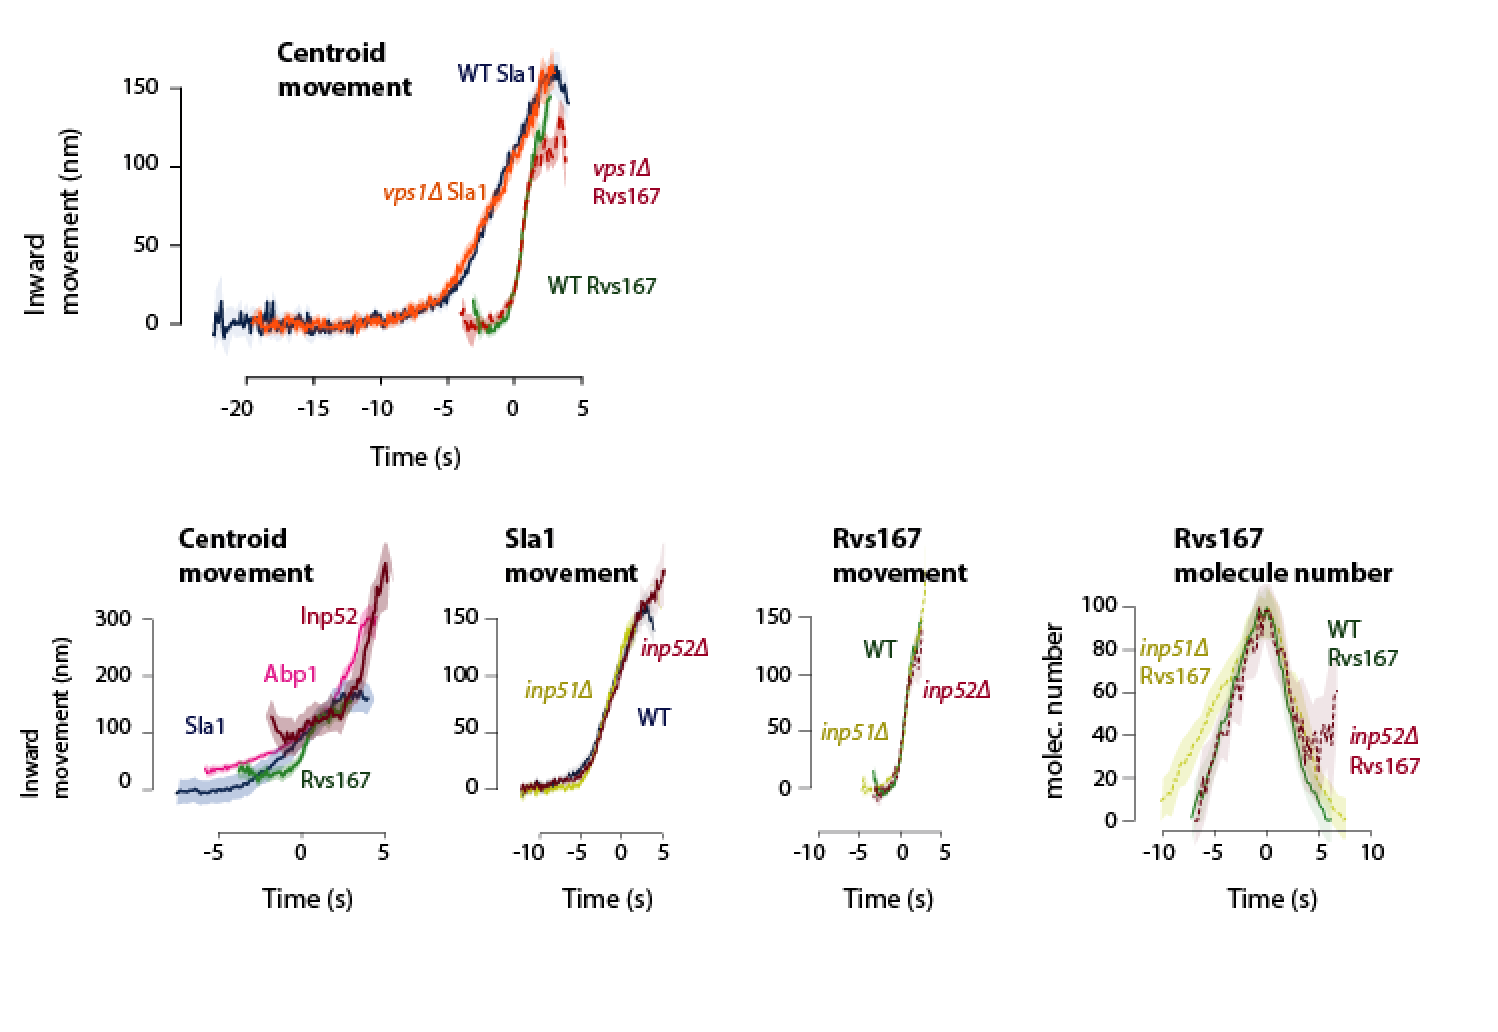
\includegraphics[width=4cm, height=4cm, keepaspectratio]{figures/vps1_placeholder}
%	\caption[Endocytic pathways in cells]
%			\label{intro_mayor}}
%\end{figure}

%\begin{wrapfigure}{l}{.46\textwidth}
%	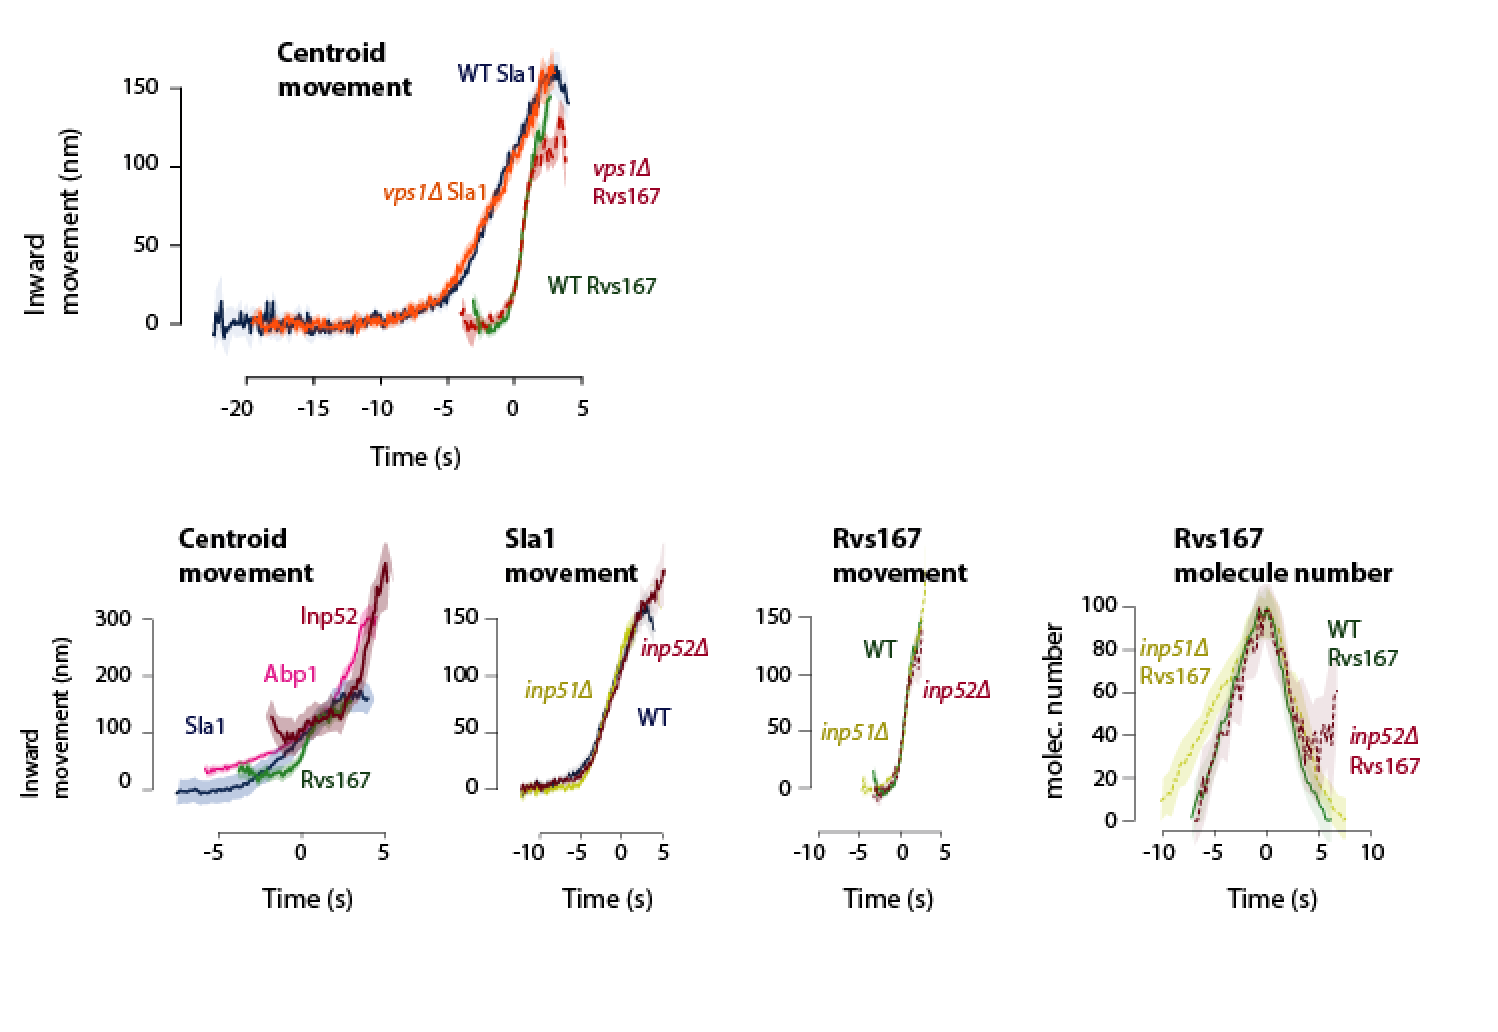
\includegraphics[width=\hsize]{figures/vps1_placeholder}
%	\caption{A half-columnwidth image using wrapfigure, to be used sparingly. Note that using a wrapfigure before a sectional heading, near other floats or page boundaries is not recommended, as it may cause interesting layout issues. Use the optional argument to wrapfigure to control how many lines of text should be set half-width alongside it.}
%	\label{fig:halfwidth}
%\end{wrapfigure}

\begin{figure}
	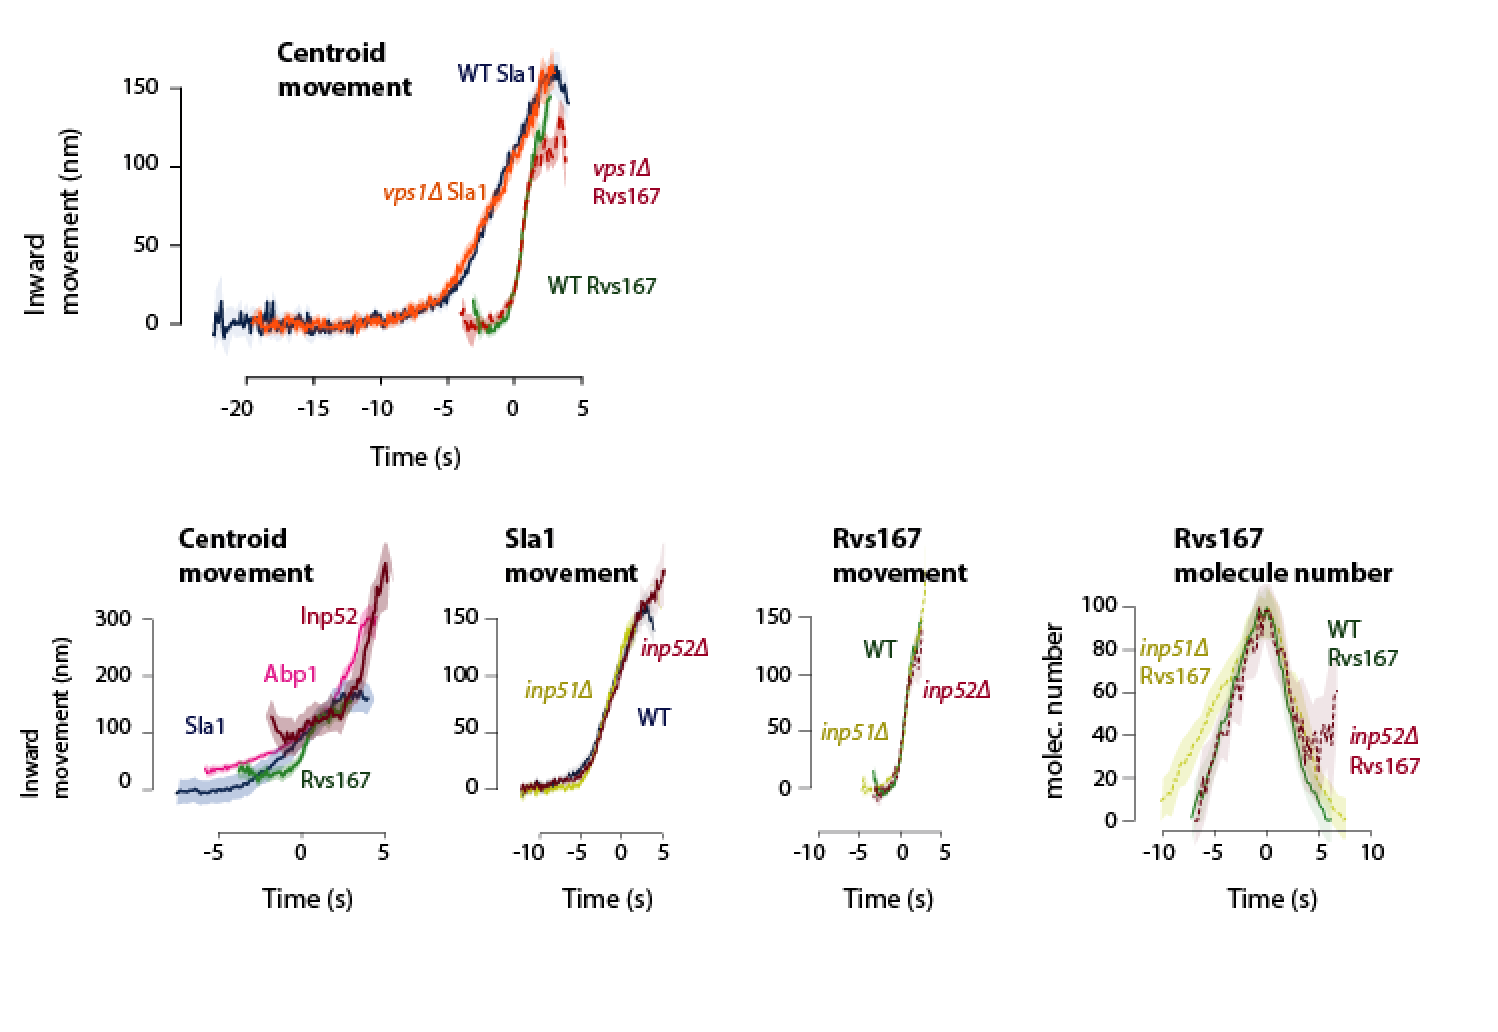
\includegraphics[width=\hsize]{figures/vps1_placeholder}
	\caption{A half-columnwidth image using wrapfigure, to be used sparingly. Note that using a wrap figure before a sectional heading, near other floats or page boundaries is not recommended, as it may cause interesting layout issues. Use the optional argument to wrapfigure to control how many lines of text should be set half-width alongside it.}
	\label{fig:halfwidth}
\end{figure}

\subsection{Rvs deletion reduces coat movement}
The Rvs complex itself is known to influence scission: deletion reduces scission efficiency by 30\% (ref1marko). Failed scission events are characterized by inward movement, followed by retraction of the coat protein Sla1 (ref1marko). Contribution of Rvs to the scission process however, is currently unclear. In the remaining 70\% of successful invaginations, inward movement of the coat protein Sla1 also deviates from the wild-type. In Fig.1, the averaged centroid trajectory (ref2andrea) of Sla1-eGFP is tracked in rvs167deletion and wild-type cells. Time alignment is established by tracking the centroid of a second protein, here m-Cherry tagged Actin binding protein Abp1. Simultaneous tracking of GFP-tagged protein of interest and m-Cherry tagged Abp1 allows us to align all other proteins to the Abp1 reference centroid (ref2andrea). Time=0, is established as the peak of the Abp1 fluorescence intensity, which in wild-type is concomitant with the peak of Rvs167 fluorescent intensity (ref2andrea, ref3wanda), and is time in which scission occurs. Sla1 centroid in rvs167deletion cells follows the wild-type centroid movement till about 60nm, after which movement slows down and scission occurs. That scission occurs at shorter invaginations lengths is confirmed by formation of smaller vesicles and shorter invagination lengths in rvs167deletion cells, quantified by Correlative light and electron microscopy (CLEM) (ref3wanda). Invagination lengths of 60nm is the time window for arrival of Rvs167 (ref3wanda), indicating that coat movement of endocytic sites in rvs167deletion cells progresses normally till the expected arrival of Rvs. 


\subsection{Rvs BAR domains recognize membrane curvature in-vivo}
The curved tertiary structure and liposome binding assays of N-BAR domains have suggested that they may have a preference for curved membrane that match their own intrinsic curvature. Alternately, they may also impose their curvature on flat membrane and induce curvature formation. In-vivo, the curvature interaction of Rvs167 has not been tested. In order to do so, we delete the SH3 domain of Rvs167 observe the localization of endogenously tagged Rvs167-eGFP and BAR-eGFP and Abp1-mCherry in WT and sla2deletion cells. Sla2 acts as the molecular linker between forces exerted by the actin network and the plasma membrane. Sla2deletion cells therefore have a polymerizing actin network, but the membrane remains flat and endocytosis fails. In these cells, the full-length Rvs167 protein co-localizes with Abp1-mCherry, indicating that it is recruited to endocytic sites. BAR-eGFP localization is removed, except for rare transient patches that do not co-localize with Abp1-mCherry. 

\subsection{Rvs SH3 domains contribute to curvature independent localization}
We have shown that BAR domains need membrane curvature to localize. Full-length Rvs167, however, is recruited to endocytic patches in sla2deletion cells. This indicates that a second interaction, that is not the BAR-curvature dependent, recruits the protein to endocytic sites. This interaction must come from the SH3 region, showing that Rvs localization is dependent on both BAR as well as SH3 domain interactions. Absense of the SH3 domain also reduces total recruitment of Rvs and Abp1 protein, giving the SH3 domain an important and surprising role in regulating the late stage of endocytosis. 

\subsection{SH3 domains are recruited by Myosin 5}
SH3 domains have been shown to interact with several proteins in the actin module of endocytosis: Las17, type I myosins, and Vrp1 all have genetic or physical interactions with Rvs167 SH3 domains (Lila and Drubin, 1997; Colwill et al., 1999, Madania et al., 1999; Liu et al., 2009). 
We tested the interaction by studying the localization of full-length Rvs167 in cells with one of these proteins deleted, and treated with Las17 to reproduce the situation in which BAR-curvature interaction is removed. 
As seen in (some figure), deletion of neither Las17 nor Myo3 in combination with LatA treatment does not remove the localization of Rvs167. Deletion of Vrp1 and Myo5, with LatA treatment removes localization of Rvs167. Since Vrp1 is required for the recruitment of Myo5 (refMyo5), SH3 domains interact with Myo5 rather than Vrp1. 
\subsubsection{\color{red} 
	what about the differences in myo5 and myo3 number... if the Rvs recruitment only slightly depended on myo3 we probably wouldnt see a difference

\subsection{N-helix and GPA domains do not contribute to recruitment of Rvs or membrane movement}
\lipsum[12]
	
\subsection{Increased BAR recruitment corresponds to increased membrane movement}
\lipsum[15]

\begin{figure}	
	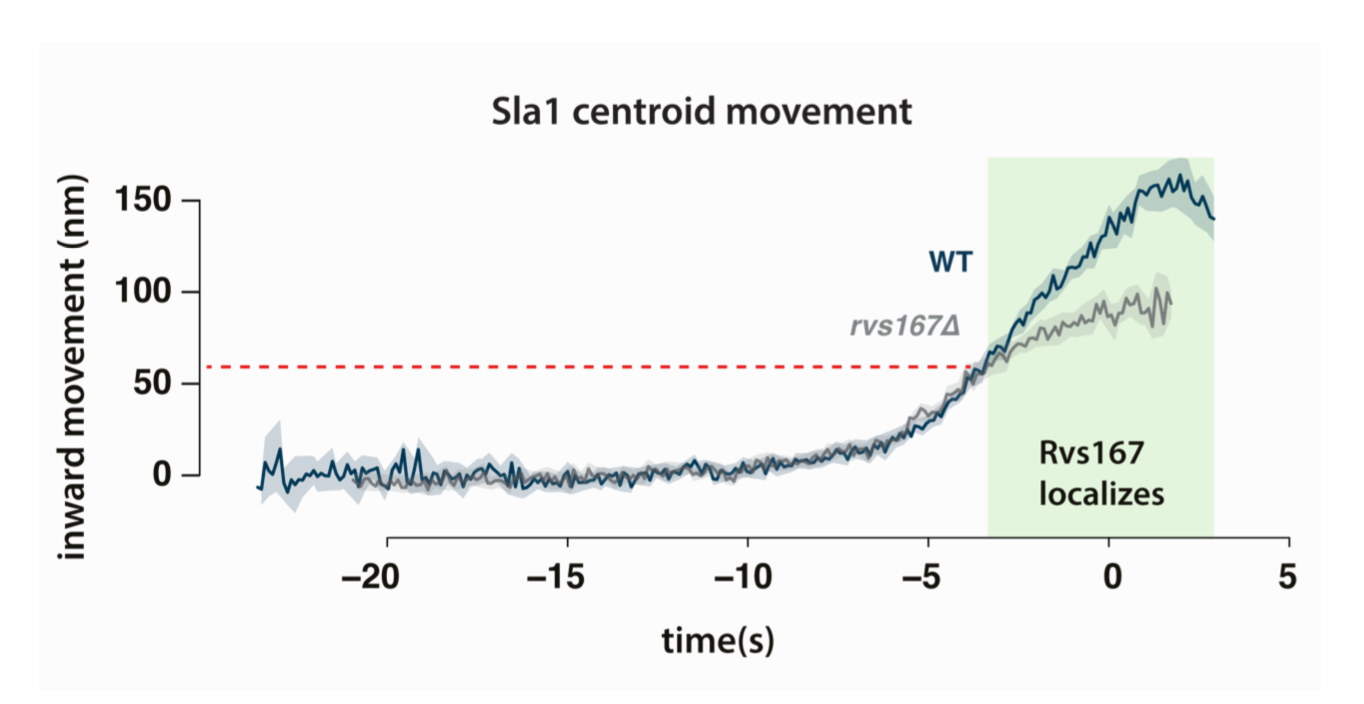
\includegraphics[
	width=0.6\textwidth,
	height=0.9\textwidth,
	keepaspectratio=true
	] {figures/rvs_del_placeholder}
	\caption{A half-columnwidth image using wrapfigure, to be used sparingly. Note that using a wrapfigure before a sectional heading, near other floats or page boundaries is not recommended, as it may cause interesting layout issues. Use the optional argument to wrapfigure to control how many lines of text should be set half-width alongside it.}
	\label{fig:halfwidth}
\end{figure}


%\begin{table}[bt]
%\caption{\label{tab:example}Automobile Land Speed Records (GR 5-10).}
% Use "S" column identifier to align on decimal point 
%\begin{tabular}{S l l l r}
%\toprule
%{Speed (mph)} & Driver          & Car                        & Engine    & Date     \\
%\midrule
%407.447     & Craig Breedlove & Spirit of America          & GE J47    & 8/5/63   \\
%413.199     & Tom Green       & Wingfoot Express           & WE J46    & 10/2/64  \\
%434.22      & Art Arfons      & Green Monster              & GE J79    & 10/5/64  \\
%468.719     & Craig Breedlove & Spirit of America          & GE J79    & 10/13/64 \\

%\end{tabular}

%\medskip 
%Source: \url{https://www.sedl.org/afterschool/toolkits/science/pdf/ast_sci_data_tables_sample.pdf}

%\tabledata{This is a description of a data source.}

%\end{table}


\section{Discussion}

\lipsum[9]

\section{Methods and Materials}

Guidelines can be included for standard research article sections, such as this one. 

\lipsum[3]





\subsection{Citations}

LaTeX formats citations and references automatically using the bibliography records in your .bib file, which you can edit via the project menu. Use the \verb|\cite| command for an inline citation, like \cite{Aivazian917}, and the \verb|\citep| command for a citation in parentheses \citep{Aivazian917}. The LaTeX template uses a slightly-modified Vancouver bibliography style. If your manuscript is accepted, the eLife production team will re-format the references into the final published form. \emph{It is not necessary to attempt to format the reference list yourself to mirror the final published form.} Please also remember to \textbf{delete the line} \verb|\nocite{*}| in the template just before \verb|\bibliography{...}|; otherwise \emph{all} entries from your .bib file will be listed! 

%\begin{featurebox}
%\caption{This is an example feature box}
%\label{box:simple}
%This is a feature box. It floats!
%\medskip

%\includegraphics[width=5cm]{example-image}
%\featurefig{`Figure' and `table' captions in feature boxes should be entered with \texttt{\textbackslash featurefig} and \texttt{\textbackslash featuretable}. They're not really floats.}

%\lipsum[1]
%\end{featurebox}




\section{Acknowledgments}

Additional information can be given in the template, such as to not include funder information in the acknowledgments section.

\nocite{*} % This command displays all refs in the bib file. PLEASE DELETE IT BEFORE YOU SUBMIT YOUR MANUSCRIPT!
\bibliography{elife-sample}

%%%%%%%%%%%%%%%%%%%%%%%%%%%%%%%%%%%%%%%%%%%%%%%%%%%%%%%%%%%%
%%% APPENDICES
%%%%%%%%%%%%%%%%%%%%%%%%%%%%%%%%%%%%%%%%%%%%%%%%%%%%%%%%%%%%


\end{document}
